\documentclass[journal,12pt,onecolumn]{IEEEtran}
\usepackage{cite}
 \usepackage{caption}
\usepackage{graphicx}
\usepackage{amsmath,amssymb,amsfonts,amsthm}
\usepackage{algorithmic}
\usepackage{graphicx}
\usepackage{textcomp}
\usepackage{xcolor}
\usepackage{txfonts}
\usepackage{listings}
\usepackage{enumitem}
\usepackage{mathtools}
\usepackage{gensymb}
\usepackage{comment}
\usepackage[breaklinks=true]{hyperref}
\usepackage{tkz-euclide} 
\usepackage{listings}
\usepackage{gvv}
%\def\inputGnumericTable{}                                 
\usepackage[latin1]{inputenc} 
\usetikzlibrary{arrows.meta, positioning}
\usepackage{xparse}
\usepackage{color}                                            
\usepackage{array}                                            
\usepackage{longtable}                                       
\usepackage{calc}                                             
\usepackage{multirow}
\usepackage{multicol}
\usepackage{hhline}                                           
\usepackage{ifthen}                                           
\usepackage{lscape}
\usepackage{tabularx}
\usepackage{array}
\usepackage{float}

\usepackage{float}
%\newcommand{\define}{\stackrel{\triangle}{=}}
\theoremstyle{remark}
\usepackage{circuitikz}
\captionsetup{justification=centering}
\usepackage{tikz}

\title{Matrices in Geometry 4.7.27}
\author{EE25BTECH11035 - Kushal B N}
\begin{document}
\vspace{3cm}
\maketitle
{\let\newpage\relax\maketitle}
\textbf{Question: }
The equation of the straight line passing through the point (3,2) and perpendicular to the line y = x is ?

\textbf{Given: } \\
The point $\vec{P}\myvec{3\\2}$ and the line $\myvec{1&-1}\myvec{x\\y} = 0$

\textbf{Solution: }\\
The general equation of a line is written as $\vec{n}^{\top}\vec{P}=c$ where $\vec{n}$ is the vector normal to the line.\\
So, $\myvec{1\\-1}$ is the direction vector for required line.\\
Hence, the normal to the required line will be 
\begin{equation}
    \vec{n} = \myvec{1\\1}
\end{equation}

As it is passing through the given point, the required equation is
\begin{equation}
    \vec{n}^{\top}\brak{\vec{x}-\myvec{3\\2}} = 0
\end{equation}

\begin{equation}
    \implies \vec{n}^{\top}\vec{x} = 5
\end{equation}
i
\textbf{Final Answer: }\\
$\therefore$The equation of the required straight line is $\myvec{1&1}\myvec{x\\y}=5$

\begin{figure}[H]
    \centering
    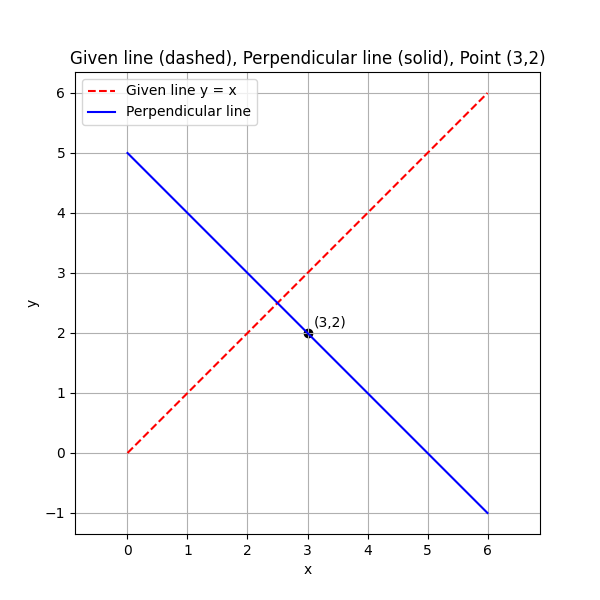
\includegraphics[width=0.55\columnwidth]{figs/2.png}
    \caption{}
\end{figure}
\end{document}

